%!TEX TS-program = pdflatex
\documentclass[acmtog]{acmart}
\usepackage{graphicx}
\usepackage{float}

\title{Recognizing Smartphone Motion Gestures Using PCA and KNN}

\author{James Chang }
\affiliation{%
  \institution{University of Penn }
  \city{Phili}
  \country{USA}}
\email{maam@author.com}

\setlength{\abovecaptionskip}{0pt}
\setlength{\belowcaptionskip}{0pt}
\usepackage{tikz}
\usetikzlibrary{arrows.meta, positioning}


\begin{document}


\begin{abstract}
The proposed method is to identify  single motions of the smartphones using  K-nearest neighbors to  classify acceleration  data in X, Y, Z. Compared to the prior work in recognizing human body motions, we do not use the data of all motions to identify differences, which is not practical in interactive applications such as mobile gaming. Instead, we  extract dominating base vectors from the subspace of each motion's covariance matrix through Principle Component Analysis (PCA) . The energy projected on the space from time series of one motion will be a metric for KNN classification.   The method has been verified in Matlab enviroment based on the samples of three different motions collected from UnityRemote, a platform for mobile gaming development.
\end{abstract}

\maketitle

\section{Introduction}
Recognizaing motions (human activities or mobile devices) is useful in different applications such as \cite{human_activity_paper}. One of the applications is for the interactive applications such as mobile gaming, where the system has to identify each single motion for characters' movement and actions. Solely rely on using buttons and scratching screens would not provide good user experience esp for ? games when characterers need to jump or take turns. It would be more intuitive to use the mobile devices to control. For this specific requirement people has to rely on the built-in accerator to track users' behaviours.
In this paper we explored the method to dentify  single motions of the smartphones using  K-nearest neighbors (KNN) to  classify acceleration  data in X, Y, Z. Compared to the prior work in recognizing human body motions \cite{matlab1}, we do not use the data of all motions to identify differences, which is not practical in interactive applications such as mobile gaming. Instead, we  extract the dominating  subspace of each motion's covariance matrix. The energy projected on the vector from samples of one motion will be a metric for KNN classification. 

The paper is organized as follows. We first introduced the previous work on recogniazing human body activity . And we would point out the limitations for moblie applicatoins. In the following session , methodology we introduced the improved algorithm to identify singe motions. The method has been verified in Matlab enviroment based on the samples of three different motions collected from UnityRemote, a platform for mobile gaming development.


\section{Related Work}
In \cite{matlab1} people used the method below to identify different human body movements \cite{human_data}. The top level flow chart is shown in  Figure \ref{fig:def_pipeline}.  There are two main steps.  The first step is to extract statistical metrics (features) from the raw data through Principle Component Analysis (PCA) \cite{pca} instead of using the raw data directly. The second step is to use KNN for classification based on features from training data.  One  measurement is a $N$ by $3$ matrix $V$  recording acceration data in directions of X Y Z for one activity, where $V$ is defined by 
\begin{equation}
V =
\begin{bmatrix}
\vec{v}_x , \vec{v}_y , \vec{v}_z
\end{bmatrix}
\label{eq:one_measure}
\end{equation}
where $\vec{v}_x=[v_{x,1},\dots,v_{x,N}]^\top$ is a time series of $N$ points recording acceration data in X direction when there is a motion happening. 
We will have multiple matrices of $V$ when we repeat each motion many times. It is more convenient to seperate three directions. We have

\begin{equation}
X =
\begin{bmatrix}
\vec{v}_{x_1} ,\dots,\vec{v}_{x_M}
\end{bmatrix}
=
\begin{bmatrix}
v_{x_{1,1}} & \dots & v_{x_{1,M}} \\
 \vdots  &\vdots & \vdots \\
v_{x_{1,N}} & \dots & v_{x_{N,M}}
\end{bmatrix}
\label{eq:multi_measure}
\end{equation}
where $X$ is a $N$ by $M$ matrix and $\vec{v}_{x_m}$ , a time series , is one of multiple samples. $M$ is the number of sampling. Similarly we will have $Y$ and $Z$ for other two directions. 

Three statistical metrics are extracted from time series as the coordinate for distance calculation later in KNN. Two of them, $u_{x_m} $ and $\sigma_{x_m}$, are mean and sigma for the time series, $\vec{v}_{x_m}$. The third one,  $e_{x_m}$, is the projection (energy) of  $\vec{v}_{x_m}$ on the dominating subspace of the motion  as described below.
First we have the covariance matrix of $X$ \cite{cov_m} defined by 
\begin{equation}
cov(X)=\frac{1}{M} (X-\bar{X})(X-\bar{X})^\top
\label{eq:cov_x}
\end{equation}
where $\bar{X}$ is defined by 
\begin{equation}
\bar{X}=
\begin{bmatrix}
v_{x_{1,1}}-u_{x,t,1} & \dots & v_{x_{1,M}}-u_{x,t,1} \\
 \vdots & \vdots & \vdots \\
v_{x_{1,N}}-u_{x,t,N} & \dots & v_{x_{N,M}}-u_{x,t,N}
\end{bmatrix}
=
\begin{bmatrix}
\vec{v}_{x_1}-\vec{u}_{x,t} ,\dots, \vec{v}_{x_M}-\vec{u}_{x,t}
\end{bmatrix}
\label{eq:mean_x}
\end{equation}
and $u_{x,t,n}$ is the mean of $M$ sampling points at the $n_{th}$ point in the time series defined by
\begin{equation}
u_{x,t,n}=\frac{1}{M}  \sum_{m=1}^{M} v_{x_{n,m}}
\label{eq:cov_x}
\end{equation}
Please note that we add $t$ to differentiate $u_{x_m}$ and $v_{x_{n,m}}$ is one element in [\ref{eq:multi_measure}].
$-\bar{X}$  is to centerize the original time series by  removing the mean. Thanks to the covariance matrix we can capture the correlation between elements in time series when we repeat the measurement many times. And the correlation would differ depending X Y Z directions as well as different motions. Figure \ref{fig:cov_cmp} shows the differences of covariance in Z direction among different motions in our measurement. The next step is  to extract the key information from the covariance matrix. We can find the dominating direction in the covariance matrix  with the help of PCA defined by
\begin{equation}
cov(X)=U \Sigma U^\top
\label{eq:pca}
\end{equation}
where $U=[\vec{u}_1, ...,\vec{u}_N]$  is the eigenvectors for the $cov(X)$ and $\Sigma$ is a diagonal matrix. Without loss of generality we define the $\vec{u}_1$ is the dominating vector, corresponding to the biggest eigenvalue  in $\Sigma$. Then $\vec{u}_1$ represents the dominating direction  to the motion in X coordinate.  The projection on $\vec{u}_1$ , defined by 
\begin{equation}
e_{x_m}=(\vec{v}_{x_m}-\vec{u}_{x,t})^\top \vec{u}_1
 \label{eq:e_on_M}
\end{equation}
where $\vec{v}_{x,t}$ is equation  \ref{eq:mean_x} and $e_{x_M}$ is the third metric along with mean and sigma of $\vec{v}_{x_m}$. Therefore we can define a function called $F(X)$ to convert matrix $X$ into $X_{KNN}$ for KNN classification, where $F(X)$ converts $N$ by $M$ matrix into a $M$ by $3$ matrix

\begin{equation}
F(X)=
X_{KNN} =
\begin{bmatrix}
u_{x_1} & \sigma_{x_1} & e_{x_1} \\
 \vdots & \vdots & \vdots \\
u_{x_M} & \sigma_{x_M} & e_{x_M} \\
\end{bmatrix}
\label{eq:f_func}
\end{equation}
We will have $F(Y)=Y_{KNN}$ and $F(Z)=Z_{KNN}$ following the similar procedure. The coordinate of  distance calculation in KNN will be $[X_{KNN} ,Y_{KNN}, Z_{KNN} ] $

It is worthy noting that it is required to generate similar matrices for testing data as well for prediction. We will have  $X_{KNN,test}$ from $F(X_{test})$ and  $[X_{KNN,test} ,Y_{KNN,test} ,Z_{KNN,test} ] $  \cite{matlab1}.

Application of the classification using KNN, a supervised machine learning method, would be straightforward where each row in \\ $[X_{KNN,test} ,Y_{KNN,test} ,Z_{KNN,test} ] $
 will be classfied based on the distance to $[X_{KNN} ,Y_{KNN}, Z_{KNN} ] $. We used K=1 and Euclidean distance.  Figure \ref{fig:def_pipeline} summarizes the high level flow of the method.
 
 The method above performs very well not only in the data \cite{human_data,matlab1} but also in our own data in the following sessions. But this method is not practical for interactive applications. The reason is that  all testing data are required to generate $e_{x_m}$ since we need  the covariance matrix of all motion data to get corresponding projection on dominating subspace/direction. In  gaming we need to detect a single motion alone. Detection all testing data together is not helpful. To solve this challenge we proposed an improved method to implement regonization of single motioins, without relying other testing data.
 
\section{Methodology and Experimental results}

The main improvement is the different method to extract $e_{x_m}$ in testing data. Figure \ref{fig:new_pipeline} provides top level pipeline. Compared with Figure \ref{fig:def_pipeline},  $e_{x_m, test}$ is not from $F(X_{test})$, covariance matrix of testing data self. Instead we project $\vec{v}_{x_m,test}$  on $\vec{u}_1$ which is from  training data,$X$, to calculate a new $e_{x_m,test}$. In other words, we obtained $e_{x_m,test}$ from the single motion self , which differs from  the  previous method. And at same time we have to use the mean vector $\vec{u}_{x,t}$, from training data as well. Note that $\vec{u}_{x,t}$ is from the entire testing data as well in the previous method . We have
\begin{equation}
e_{x_m,new}=(\vec{v}_{x_m}-\vec{u}_{x,t,train,mean})^\top \vec{u}_{1,train}
 \label{eq:e_on_M_new}
\end{equation}
where we add $train$ to differentiate training data and testing data and $mean$ to differentiate vector $u$

We verified the  method using the data collected from UnityRemote and Matlab scripts. First we use \textsc{update} function   and \textsc{acceleration} class \cite{unity} in Unity/UnityRemove to capture data on X/Y/Z when we shake the phone once (Jump), rotate the phone like a wheel (Wheel) or like a key (Rotate) shown in Figure \ref{fig:motion}. We repeat 40 times for each motion. Fig \ref{fig:one_example} shows all data when Jump is repeated.  Fig \ref{fig:rotate} and \ref{fig:wheel}  shows all data for Wheel and Rotate .~10 percent random picked data are used for testing while the other is for training. We make sure all data are being tested. There is only one failure case shown in Figure \ref{fig:one_example} , which is not identified correctly.

\section{Conclusions}
The paper proposed a method to recognize single motions based on acceration data from mobile devices. The high accuracy is achieved by introduction of dominating subspace in covariance matrix of motions and usage of the projection on the subspace as the coordinate for distance calculation in KNN. Such methods would be more promising for computing due to less data size and linear operations. Implentation of such algorithms in the real applications such as interactive gaming would be the next steps.

\begin{figure}[t]
  \centering
  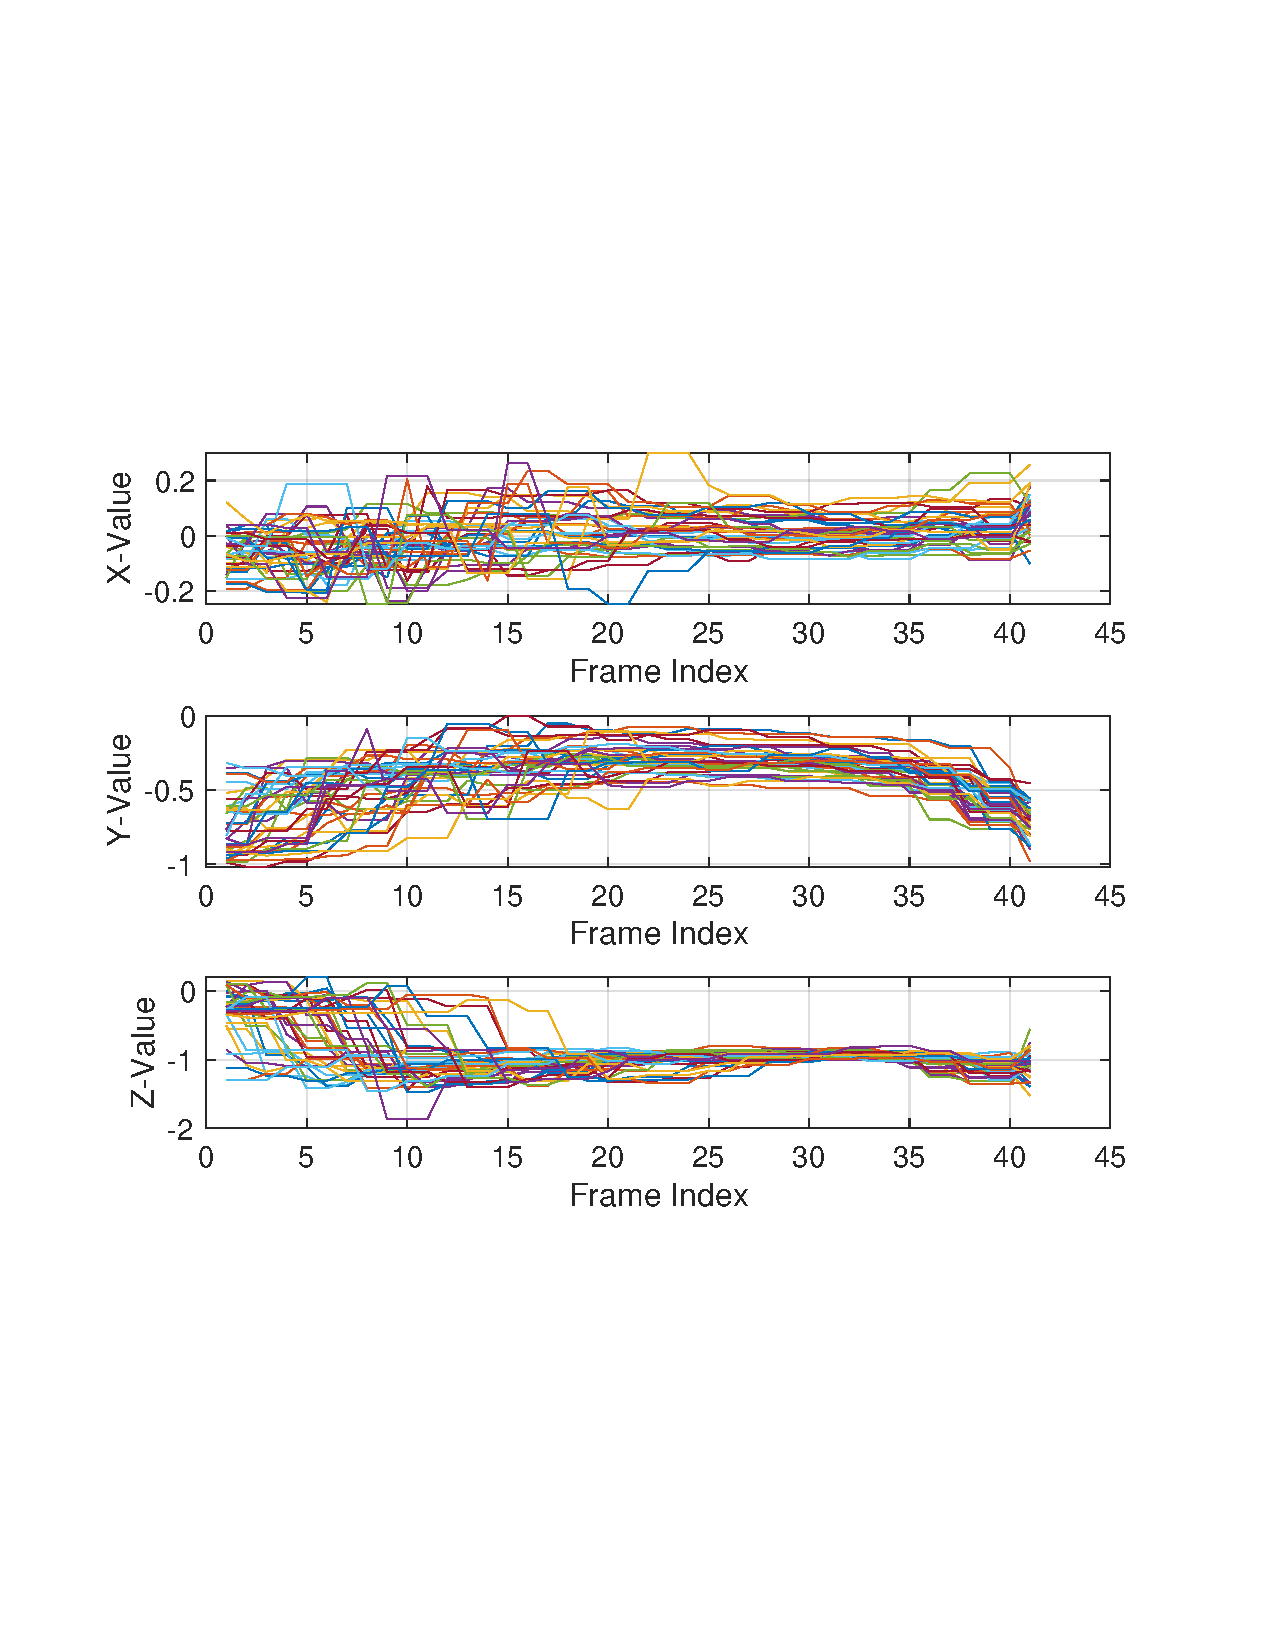
\includegraphics[width=\linewidth]{rotate.pdf}
  \caption{Multiple measurement of acceratoin data at X, Y, Z in rotate motion}
 \label{fig:rotate}
\end{figure}


\begin{figure}[t]
  \centering
  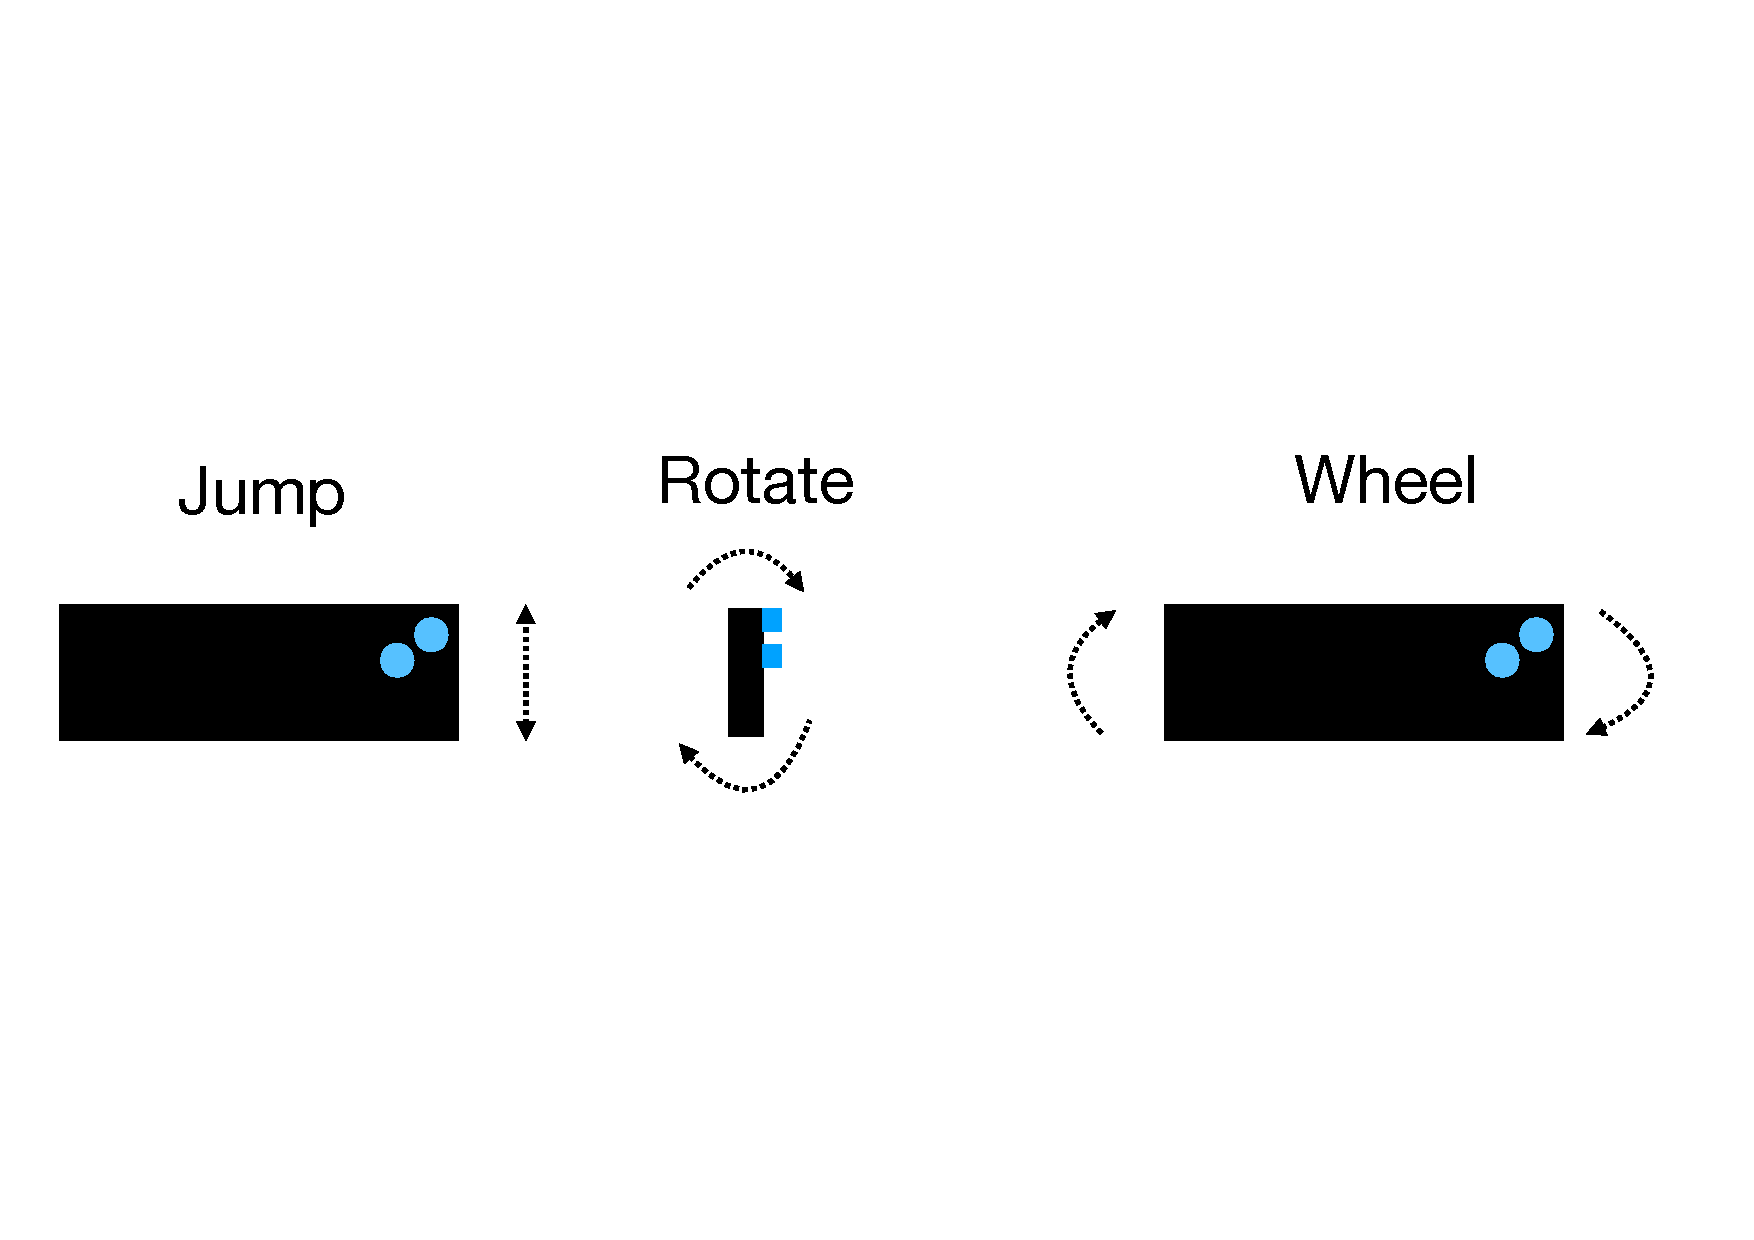
\includegraphics[width=\linewidth]{motion.pdf}
   \caption{ Motions: Jump, Wheel and Rotate}
  \label{fig:motion}
\end{figure}

\begin{figure}[t]
  \centering
  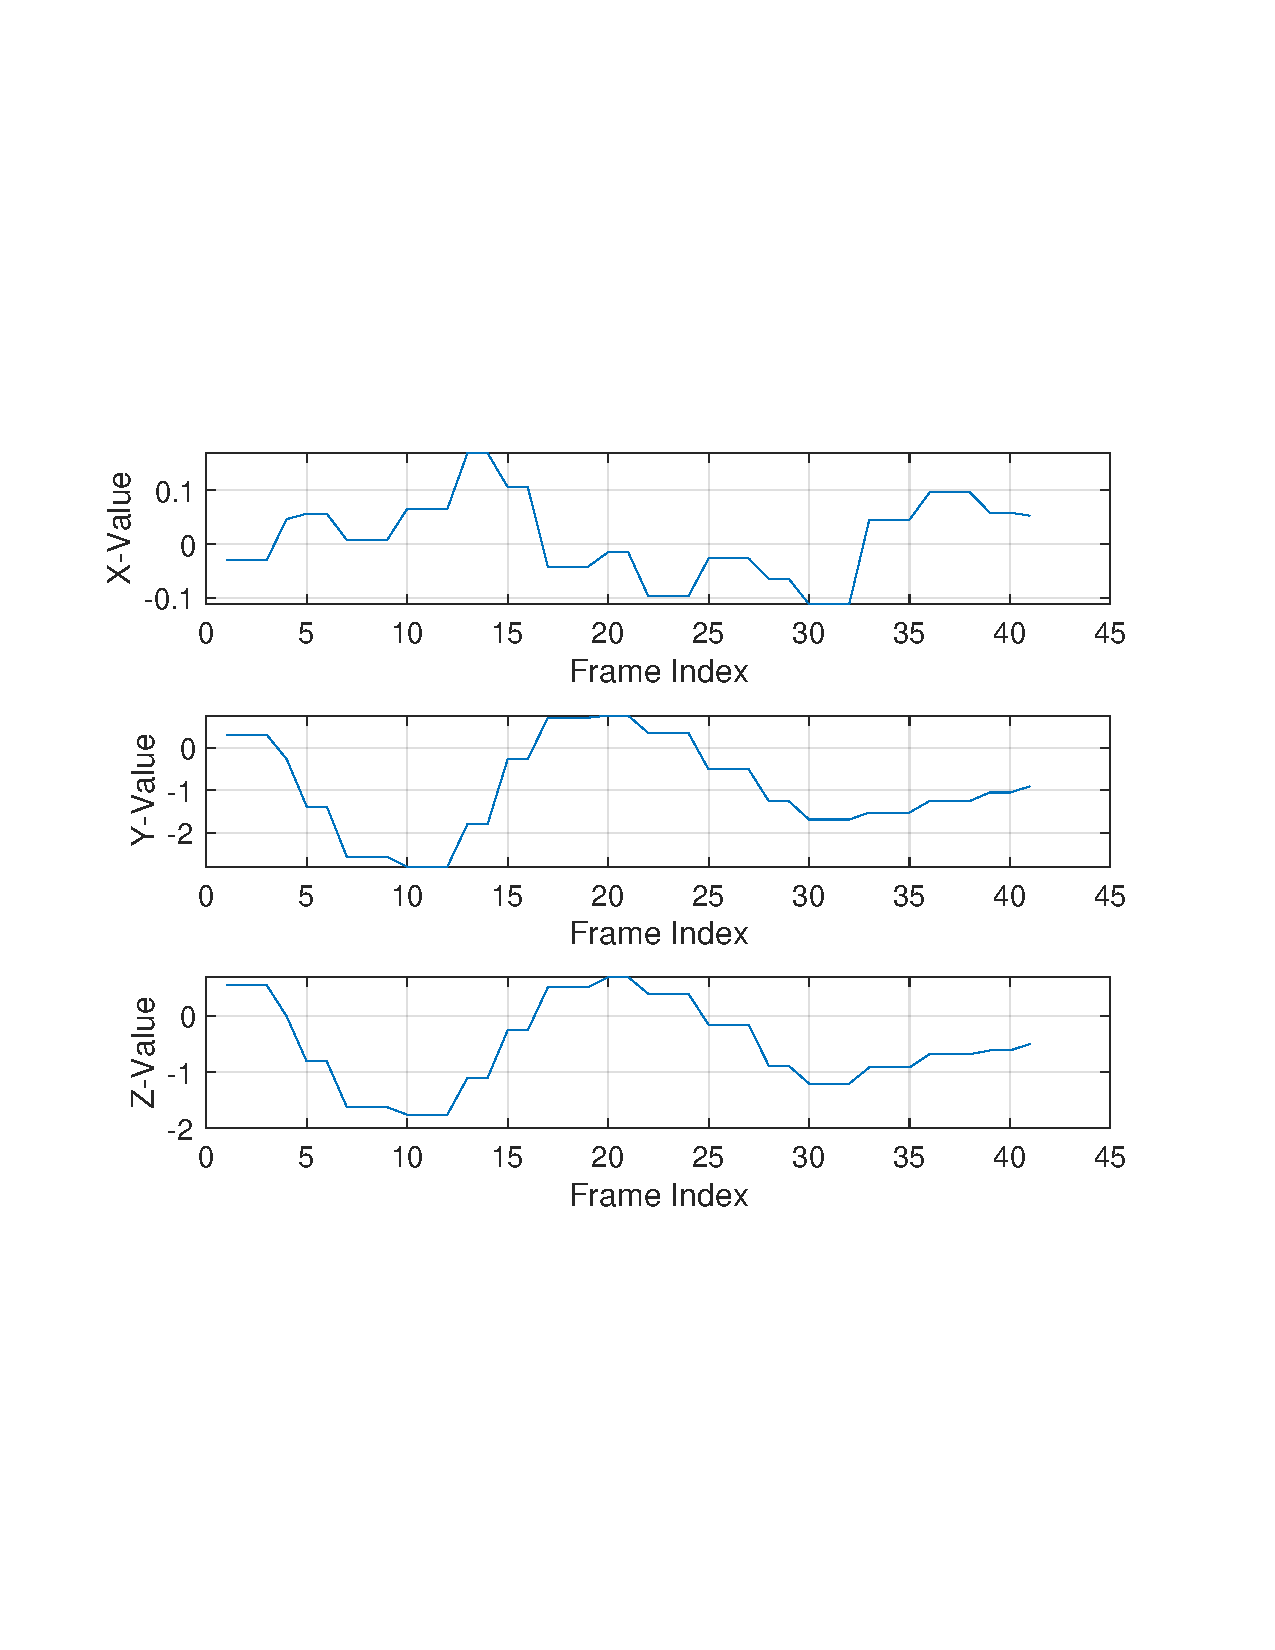
\includegraphics[width=\linewidth]{one_example.pdf}
   \caption{one measurement of acceratoin data at X, Y, Z in Jump motion}
  \label{fig:jump}
\end{figure}

\begin{figure}[t]
  \centering
  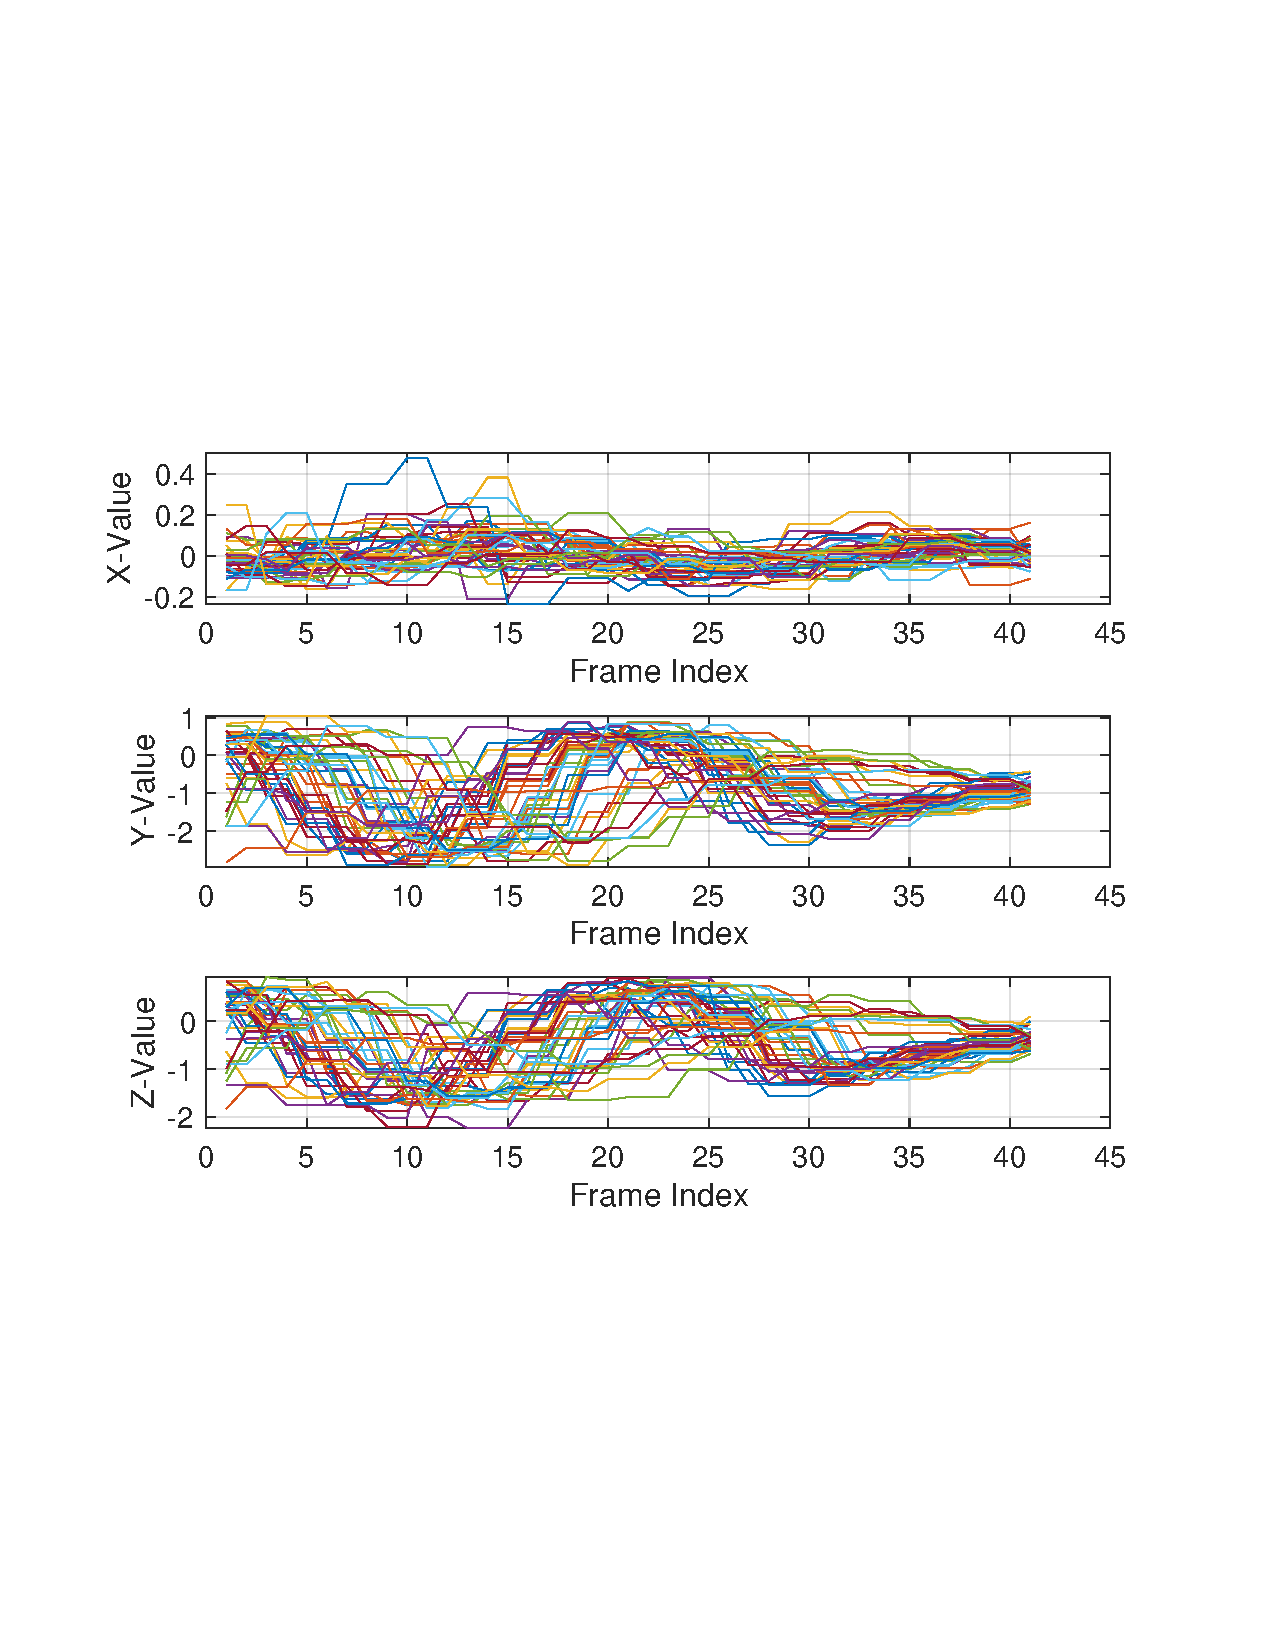
\includegraphics[width=\linewidth]{jump.pdf}
   \caption{Multiple measurement of acceratoin data at X, Y, Z in Jump motion}
  \label{fig:one_example}
\end{figure}



\begin{figure}[t]
  \centering
  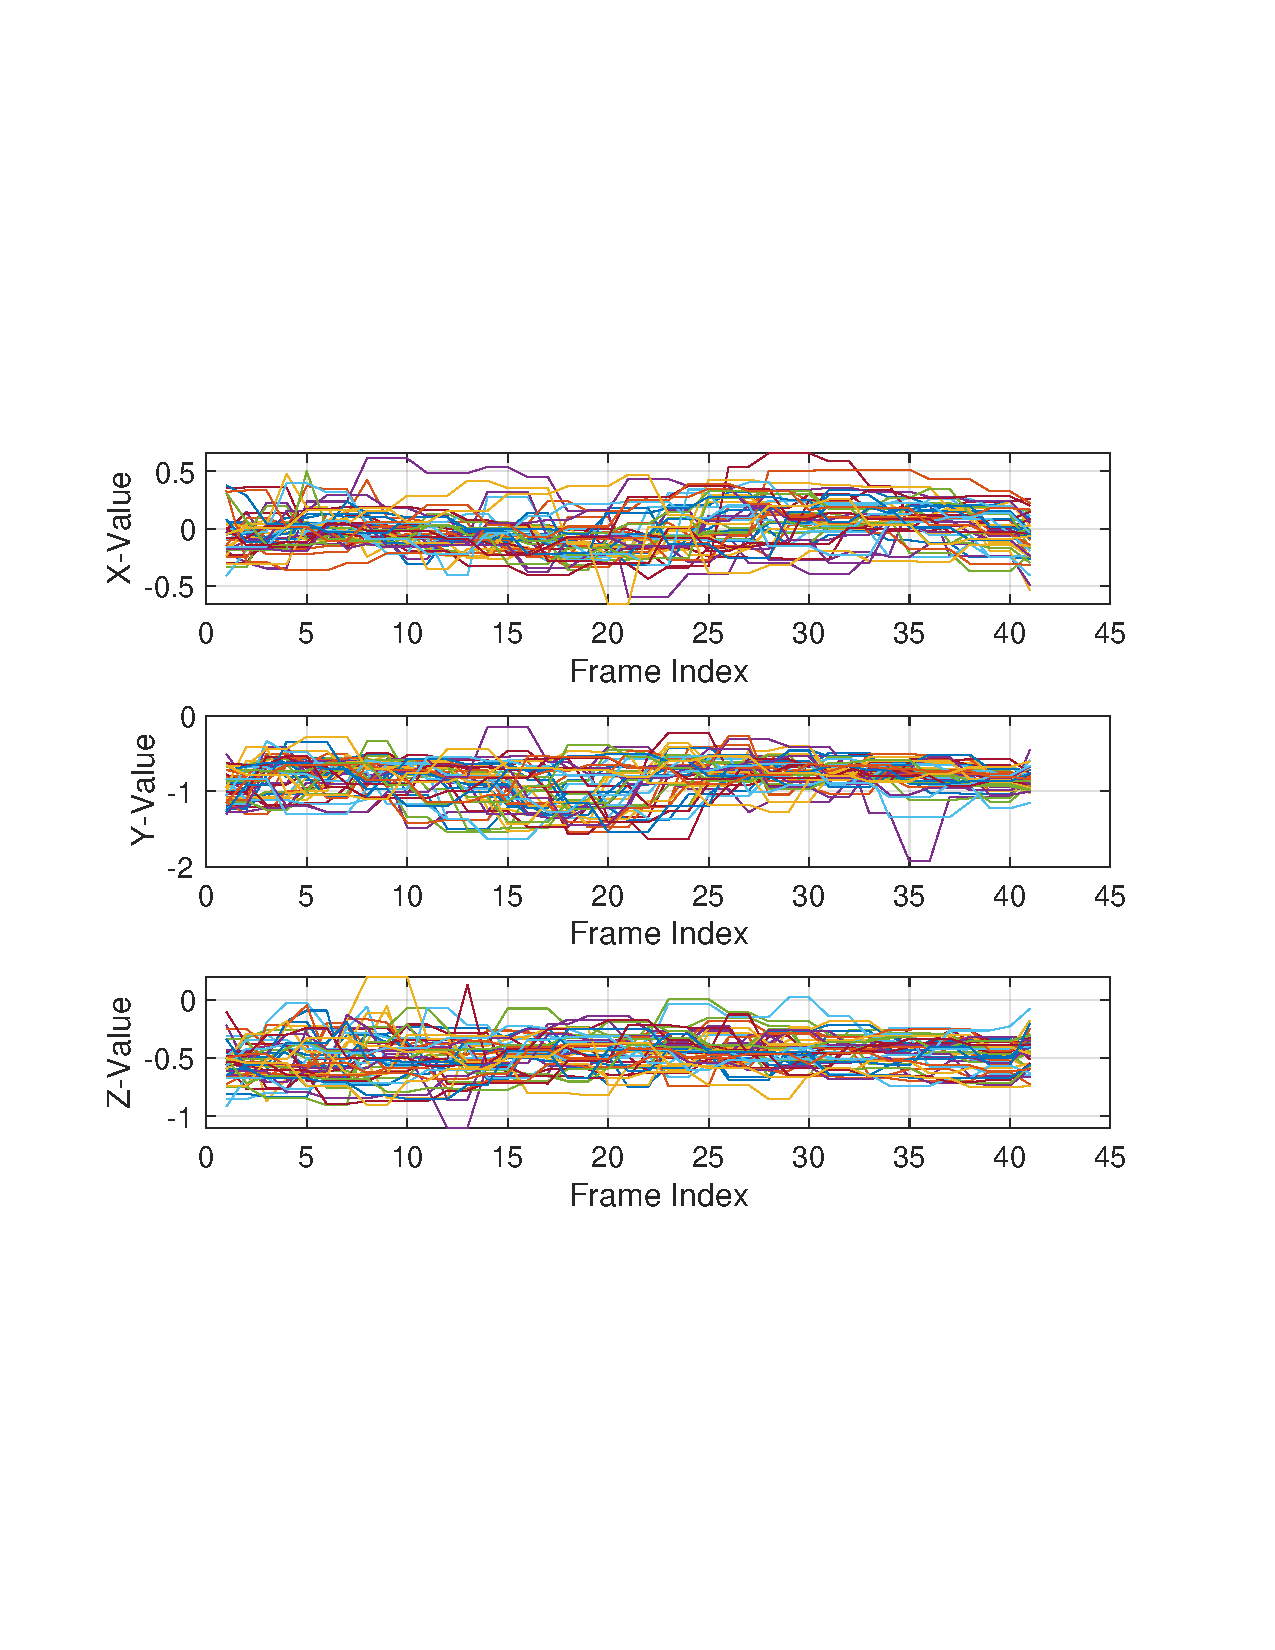
\includegraphics[width=\linewidth]{wheel.pdf}
   \caption{Multiple measurement of acceratoin data at X, Y, Z in wheel motion}
  \label{fig:wheel}
\end{figure}

\begin{figure}[t]
  \centering
  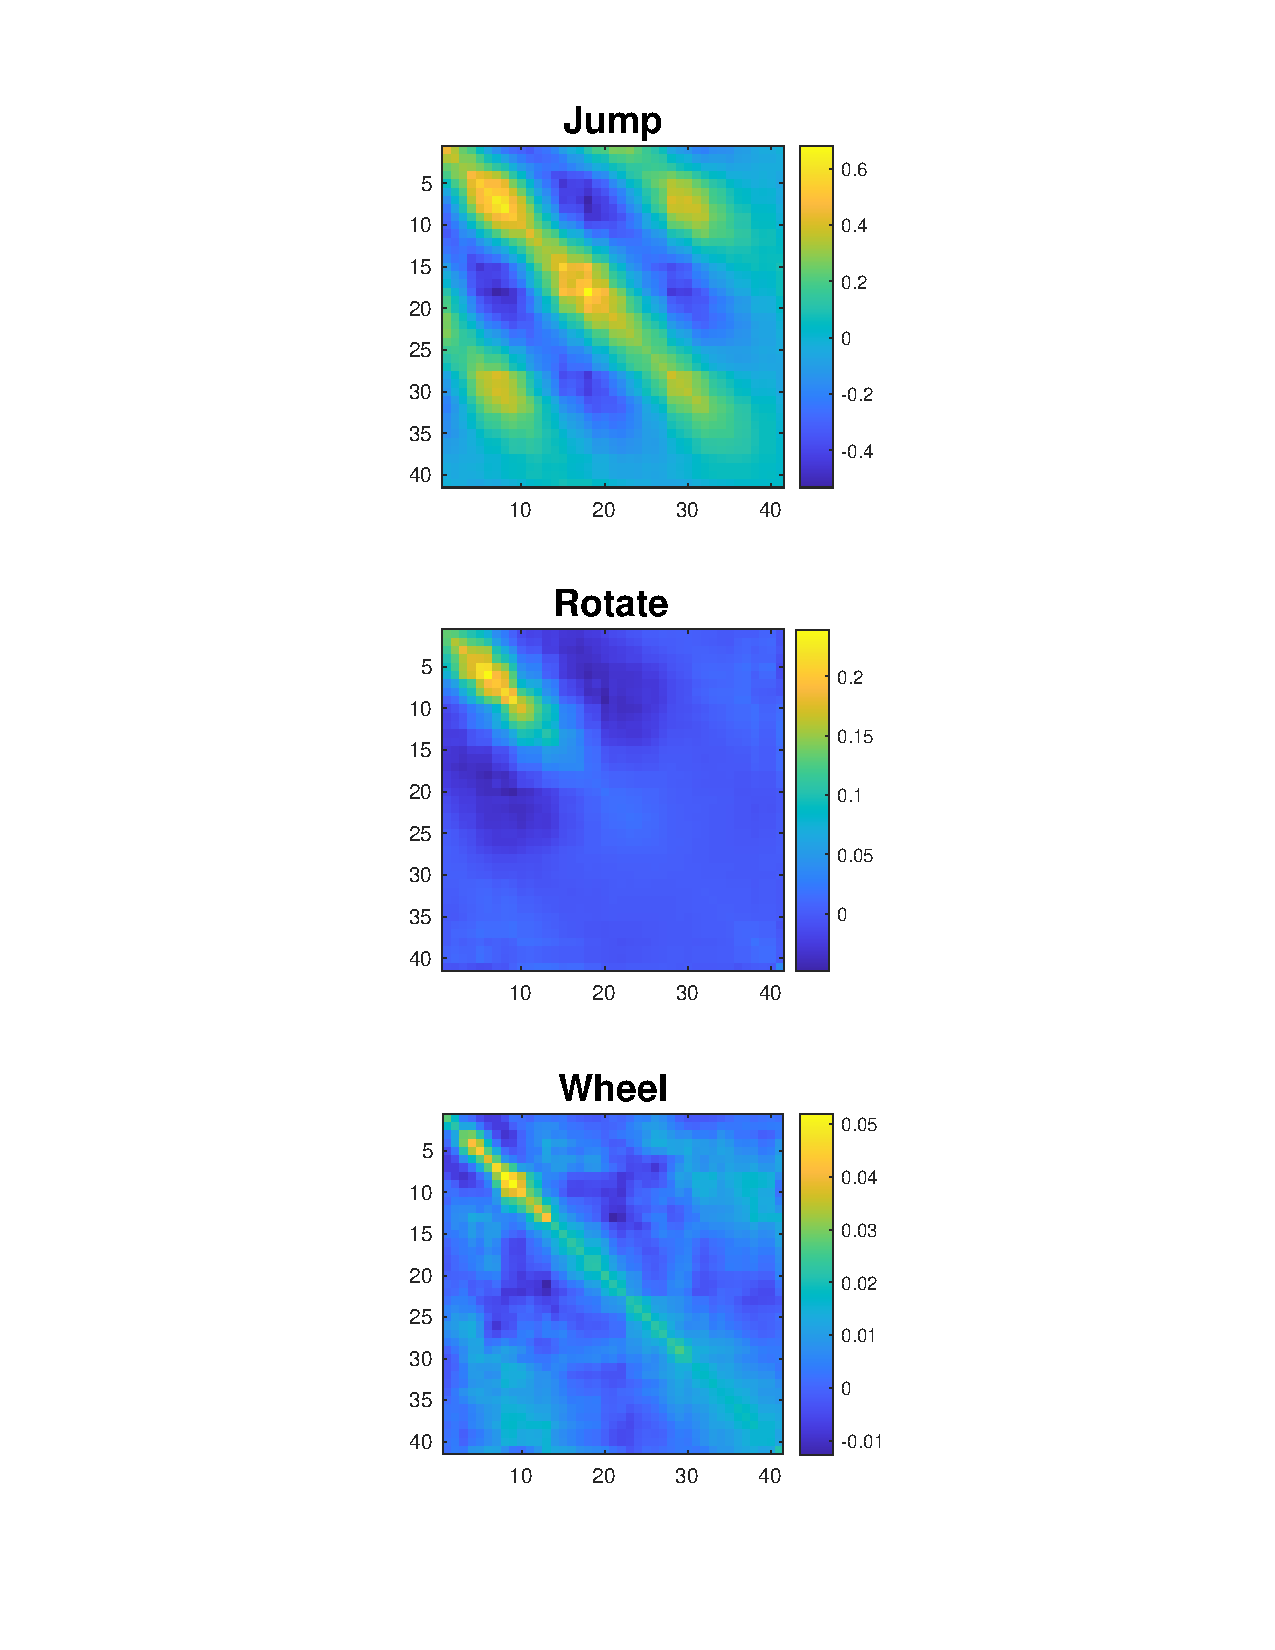
\includegraphics[width=\linewidth]{cov_compare.pdf}
   \caption{Compare covariance matrix at Z direction among three motions}
  \label{fig:cov_cmp}
\end{figure}


\begin{figure}[H]
\centering
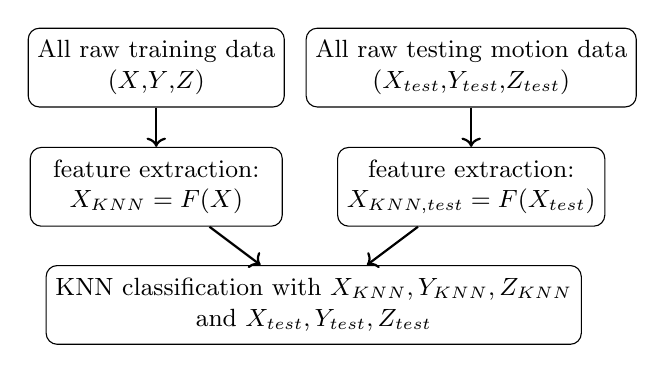
\begin{tikzpicture}[
  block/.style={
    draw, rectangle, rounded corners,
    minimum height=1cm, minimum width=3.2cm,
    align=center, font=\small
  },
  arrow/.style={->, thick}
]
\node[block,xshift=-2cm] (b1) {All raw training data \\
 ($X$,$Y$,$Z$)};
\node[block,xshift=2cm] (b2) {All raw testing motion data \\
($X_{test}$,$Y_{test}$,$Z_{test}$)};
\node[block, below=0.5cm of b1] (c1) {feature extraction: \\
 $X_{KNN}=F(X)$};
\node[block, below=0.5cm of b2] (c2) {feature extraction:\\
 $X_{KNN,test}=F(X_{test})$};
\node[block, below=2cm of b1,xshift=2cm] (merge) {KNN classification with $X_{KNN},Y_{KNN},Z_{KNN}$\\
and $X_{test},Y_{test},Z_{test}$};
\draw[arrow] (b1) -- (c1);
\draw[arrow] (b2) -- (c2);
\draw[arrow] (c2) -- (merge);
\draw[arrow] (c1) -- (merge);
  \end{tikzpicture}
 \caption{The pipeline of the previous work to recognize motions together}
  \label{fig:def_pipeline}
\end{figure}

\begin{figure}[H]
\centering
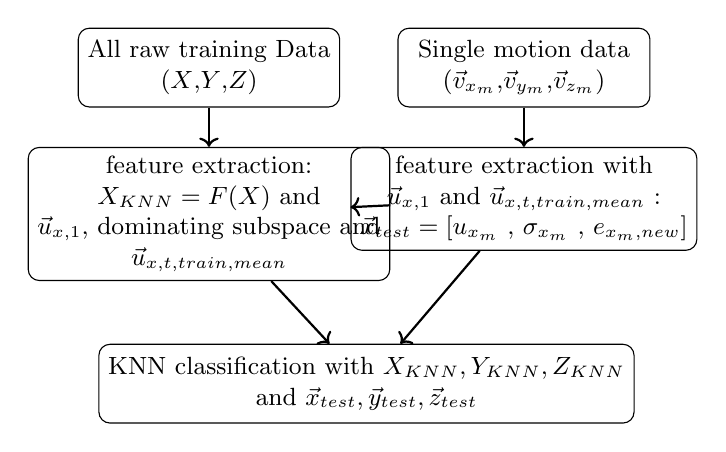
\begin{tikzpicture}[
  block/.style={
    draw, rectangle, rounded corners,
    minimum height=1cm, minimum width=3.2cm,
    align=center, font=\small
  },
  arrow/.style={->, thick}
]
\node[block,xshift=-2cm] (b1) {All raw training Data \\
($X$,$Y$,$Z$)};
\node[block,xshift=2cm] (b2) {Single motion data\\
($\vec{v}_{x_m}$,$\vec{v}_{y_m}$,$\vec{v}_{z_m}$)};
\node[block, below=0.5cm of b1] (c1) {feature extraction: \\
 $X_{KNN}=F(X)$ and \\
 $\vec{u}_{x,1}$, dominating subspace and \\
 $\vec{u}_{x,t,train,mean}$};
\node[block, below=0.5cm of b2] (c2) {feature extraction with \\
$\vec{u}_{x,1}$ and  $\vec{u}_{x,t,train,mean}$ :\\
$\vec{x}_{test}=[u_{x_m}$ ,  $\sigma_{x_m}$ , $e_{x_m,new}$]};
\node[block, below=3cm of b1,xshift=2cm] (merge) {KNN classification with $X_{KNN},Y_{KNN},Z_{KNN}$\\
and $\vec{x}_{test},\vec{y}_{test},\vec{z}_{test}$};
\draw[arrow] (b1) -- (c1);
\draw[arrow] (b2) -- (c2);
\draw[arrow] (c2) -- (merge);
\draw[arrow] (c1) -- (merge);
\draw[arrow] (c1) -- (c2);
\end{tikzpicture}
 \caption{The proposed pipeline  to recognize a single motion }
 \label{fig:new_pipeline}
\end{figure}



\bibliographystyle{ACM-Reference-Format}
\bibliography{references}

\end{document}
